% =====================================================================
\section{Practice Problems with Complete Solutions}\label{ch:practice}
% =====================================================================

The problems follow the patterns of the slides: sketching and matching vector
fields (Example~7.1, Exercises~1--3), computing gradient fields
(Example~7.2), the component test in the plane and in space
(Examples~7.4--7.5) and the three-step potential method (Example~7.6,
Exercise~4). Problems marked $(*)$ go further. Try each problem before reading
its solution.

% ---------------------------------------------------------------------
\subsection{Sketching, describing and matching vector fields}

\begin{problem}\label{q:sketch}
Sketch $\vF(x,y)=\frac12x\,\vi+\frac12y\,\vj$ at the points $(\pm1,0)$, $(0,\pm1)$,
$(\pm1,\pm1)$ and $(\pm2,0)$, and describe the field.
\end{problem}
\begin{solution}
$\vF(x,y)=\frac12\ip{x,y}=\frac12\vx$:
\begin{center}
\renewcommand{\arraystretch}{1.2}
\begin{tabular}{cccccc}
\toprule
$(x,y)$ & $(1,0)$ & $(0,1)$ & $(1,1)$ & $(-1,1)$ & $(2,0)$\\
$\vF$ & $\ip{\frac12,0}$ & $\ip{0,\frac12}$ & $\ip{\frac12,\frac12}$ & $\ip{-\frac12,\frac12}$ & $\ip{1,0}$\\
\bottomrule
\end{tabular}
\end{center}
(and symmetrically at the other points, e.g. $\vF(-1,0)=\ip{-\frac12,0}$,
$\vF(-1,-1)=\ip{-\frac12,-\frac12}$). Every arrow points directly away from the
origin (it is a positive multiple of the position vector) and has length
$\frac12r$: a \emph{radial outward} field growing linearly with distance, like the
orange panel of Exercise~2.
\end{solution}

\begin{problem}\label{q:saddle}
Describe the field $\vF(x,y)=\ip{x,-y}$. Where is it horizontal? vertical? zero?
\end{problem}
\begin{solution}
$\vF=\vzero$ only at the origin. On the $x$-axis ($y=0$), $\vF=\ip{x,0}$ is
horizontal and points \emph{away} from the origin; on the $y$-axis ($x=0$),
$\vF=\ip{0,-y}$ is vertical and points \emph{toward} the origin. In the first
quadrant arrows point right and down, etc. Length $\norm{\vF}=\sqrt{x^2+y^2}=r$.
The picture is a ``saddle'' flow: in along the $y$-axis, out along the
$x$-axis, following the hyperbolas $xy=\text{const}$. (It is
$\grad\left(\frac12x^2-\frac12y^2\right)$.)
\end{solution}

\begin{problem}\label{q:match}
Match the fields with the plots I--IV of Figure~\ref{fig:matchpractice}.\\
A. $\vF=\ip{y,-x}$\qquad B. $\vF=\ip{2,1}$\qquad C. $\vF=\ip{x,-y}$\qquad D. $\vF=\ip{y,0}$
\end{problem}

\begin{figure}[H]
  \centering
  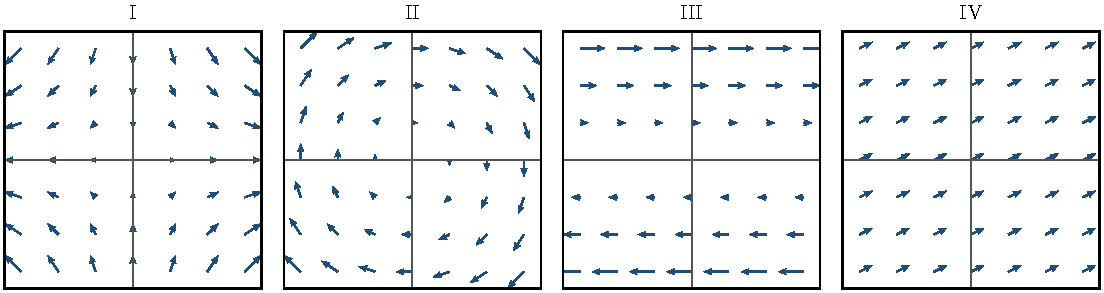
\includegraphics[width=\linewidth]{matching_practice}
  \caption{Plots for Problem~\ref{q:match}.}
  \label{fig:matchpractice}
\end{figure}

\begin{solution}
\begin{itemize}
\item B is constant: all arrows identical. Only plot \textbf{IV}.
\item D $=\ip{y,0}$ is always horizontal, pointing right above the $x$-axis and
      left below it, zero on it, longer farther from it. Plot \textbf{III}.
\item A $=\ip{y,-x}$ satisfies $\vF\cdot\vx=xy-yx=0$: tangent to circles. At
      $(0,1)$ it is $\ip{1,0}$ (to the right), so the rotation is
      \emph{clockwise}. Plot \textbf{II}.
\item C $=\ip{x,-y}$ is the saddle flow of Problem~\ref{q:saddle}. Plot \textbf{I}.
\end{itemize}
Answer: A--II, B--IV, C--I, D--III.
\end{solution}

\begin{problem}\label{q:3d}
Describe the vector field $\vF(x,y,z)=\ip{x,y,0}$ in space.
\end{problem}
\begin{solution}
Every arrow is horizontal (no $\vk$-component). At $(x,y,z)$ the arrow $\ip{x,y,0}$
points directly away from the $z$-axis, with length $\sqrt{x^2+y^2}$, the
distance to the $z$-axis. The field is the same in every horizontal plane: in
each plane $z=c$ it looks like the radial field $\ip{x,y}$. (Compare Exercise~3,
where the extra constant upward component $3\vk$ tilts every arrow upward.)
\end{solution}

% ---------------------------------------------------------------------
\subsection{Gradient fields}

\begin{problem}\label{q:grad1}
Find the gradient vector field of (a) $f(x,y)=xe^{xy}$;
(b) $f(x,y,z)=x\cos\left(\dfrac yz\right)$.
\end{problem}
\begin{solution}
\textbf{(a)} Product and chain rule: $f_x=e^{xy}+x\cdot ye^{xy}=(1+xy)e^{xy}$,
$f_y=x\cdot xe^{xy}=x^2e^{xy}$. So $\grad f=\ip{(1+xy)e^{xy},\;x^2e^{xy}}$.

\textbf{(b)} $f_x=\cos\frac yz$;
$f_y=x\cdot\left(-\sin\frac yz\right)\cdot\frac1z=-\frac xz\sin\frac yz$;
$f_z=x\cdot\left(-\sin\frac yz\right)\cdot\left(-\frac{y}{z^2}\right)=\frac{xy}{z^2}\sin\frac yz$. Hence
\[
  \grad f=\ip{\cos\frac yz,\;-\frac xz\sin\frac yz,\;\frac{xy}{z^2}\sin\frac yz}.
\]
\end{solution}

\begin{problem}\label{q:grad2}
Let $f(x,y)=x^2-y^2$. Find $\grad f$, show that it is perpendicular to the level
curve $f=3$ at $(2,1)$, and identify the field among those of
Problem~\ref{q:match}.
\end{problem}
\begin{solution}
$\grad f=\ip{2x,-2y}$, so $\grad f(2,1)=\ip{4,-2}$. The level curve $x^2-y^2=3$ passes
through $(2,1)$; implicit differentiation gives $2x-2yy'=0$, $y'=x/y=2$, so a
tangent vector is $\ip{1,2}$, and $\ip{4,-2}\cdot\ip{1,2}=4-4=0$.\checkok\
$\grad f=2\ip{x,-y}$ is twice field C (plot~I): the saddle flow.
\end{solution}

% ---------------------------------------------------------------------
\subsection{Testing for conservative fields}

\begin{problem}\label{q:which}
Which of the following are conservative?\\
(a) $\ip{y,x}$\quad (b) $\ip{y,-x}$\quad (c) $\ip{2x,2y,2z}$\quad (d) $\ip{z,0,-x}$\quad
(e) $\ip{e^x\cos y,\,e^x\sin y}$\quad (f) $\ip{e^x\cos y,\,-e^x\sin y}$
\end{problem}
\begin{solution}
\begin{enumerate}[label=(\alph*)]
\item $M_y=1=N_x$: conservative ($f=xy$).
\item $M_y=1$, $N_x=-1$: \textbf{not} conservative.
\item All cross partials are $0$: conservative ($f=x^2+y^2+z^2$).
\item $P_x=-1$ but $M_z=1$: \textbf{not} conservative.
\item $M_y=-e^x\sin y$, $N_x=e^x\sin y$: these differ wherever $\sin y\neq0$, so
      \textbf{not} conservative.
\item $M_y=-e^x\sin y=N_x$: conservative ($f=e^x\cos y$).
\end{enumerate}
\end{solution}

\begin{problem}\label{q:notcons3}
Show that $\vF=\ip{xyz^2,\;x^2yz^2,\;x^2y^2z}$ is not conservative.
\end{problem}
\begin{solution}
$M_y=xz^2$ while $N_x=2xyz^2$. These are not identically equal (at $(1,0,1)$:
$1\neq0$). One failed condition is enough: $\vF$ is not conservative. (The
other conditions need not be checked; in fact $N_z=2x^2yz=P_y$ holds, which
shows that \emph{all three} must be verified before concluding ``conservative''.)
\end{solution}

\begin{problem}\label{q:const}
(a) Find the value of $a$ for which $\vF=\ip{3x^2y+ay,\;x^3+2x}$ is conservative.
(b) Find $a,b$ such that $\mathbf{G}=\ip{yz,\;axz,\;bxy+2z}$ is conservative.
\end{problem}
\begin{solution}
\textbf{(a)} $M_y=3x^2+a$ and $N_x=3x^2+2$, equal for all $(x,y)$ iff $a=2$. Then
$\vF=\grad(x^3y+2xy)$.

\textbf{(b)} $M_y=z$, $N_x=az\Rightarrow a=1$. $N_z=ax$, $P_y=bx\Rightarrow b=a=1$.
$P_x=by$, $M_z=y\Rightarrow b=1$. All consistent: $a=b=1$, and then $\mathbf{G}=\grad(xyz+z^2)$
(Problem~\ref{q:pot3a}).
\end{solution}

\begin{problem}[$*$]\label{q:radial2d}
Let $\vF=\dfrac{\ip{x,y}}{x^2+y^2}$ on the punctured plane. Show that $M_y=N_x$ and
that, unlike the vortex field of Example~\ref{ex:vortex}, this field \emph{is}
conservative on the whole punctured plane.
\end{problem}
\begin{solution}
$M_y=\dfrac{-2xy}{(x^2+y^2)^2}=N_x$. A potential defined on the entire punctured
plane is $f=\frac12\ln(x^2+y^2)$: $f_x=\frac{x}{x^2+y^2}$, $f_y=\frac{y}{x^2+y^2}$.\checkok\
So on a non-simply-connected region the component test is inconclusive: it
holds for both fields, but one is conservative and the other is not. To prove
conservativeness there, exhibit a potential.
\end{solution}

% ---------------------------------------------------------------------
\subsection{Finding potential functions}

\begin{problem}\label{q:pot2a}
Show that $\vF=\ip{2x-3y,\;-3x+4y-8}$ is conservative and find a potential.
\end{problem}
\begin{solution}
\step{1}{Test.} $M_y=-3=N_x$ (polynomials, continuous on $\R^2$): conservative.
\step{2}{Integrate in $x$.} $f=x^2-3xy+g(y)$.
\step{3}{Match $f_y$.} $f_y=-3x+g'(y)=-3x+4y-8\Rightarrow g'(y)=4y-8\Rightarrow g=2y^2-8y+K$.

\textbf{Answer.} $f=x^2-3xy+2y^2-8y+K$. Check: $f_x=2x-3y$\checkok, $f_y=-3x+4y-8$\checkok.
\end{solution}

\begin{problem}\label{q:pot2b}
Find a potential for $\vF=\ip{(1+xy)e^{xy},\;x^2e^{xy}}$.
\end{problem}
\begin{solution}
\step{1}{Test.} $M_y=xe^{xy}+(1+xy)xe^{xy}=(2x+x^2y)e^{xy}$;
$N_x=2xe^{xy}+x^2ye^{xy}=(2x+x^2y)e^{xy}$. Equal: conservative.
\step{2}{Integrate the \emph{easier} component.} Integrating $N$ in $y$ is easier
than $M$ in $x$: $f=\int x^2e^{xy}\,\dd y=xe^{xy}+g(x)$.
\step{3}{Match $f_x$.} $f_x=e^{xy}+xye^{xy}+g'(x)=(1+xy)e^{xy}\Rightarrow g'(x)=0$.

\textbf{Answer.} $f=xe^{xy}+K$ (compare Problem~\ref{q:grad1}(a)).
\emph{Tip:} the order of the three steps may be changed; start with whichever
component is easiest to integrate.
\end{solution}

\begin{problem}\label{q:pot2c}
Find a potential for $\vF=\ip{ye^x+\sin y,\;e^x+x\cos y}$.
\end{problem}
\begin{solution}
Test: $M_y=e^x+\cos y=N_x$. Integrate in $x$: $f=ye^x+x\sin y+g(y)$. Then
$f_y=e^x+x\cos y+g'(y)=N\Rightarrow g'(y)=0$. Answer: $f=ye^x+x\sin y+K$.
\end{solution}

\begin{problem}\label{q:pot2d}
Find a potential for $\vF=\ip{\ln y+2xy^3,\;3x^2y^2+\dfrac xy}$, $y>0$.
\end{problem}
\begin{solution}
Test: $M_y=\frac1y+6xy^2$, $N_x=6xy^2+\frac1y$: equal, and the half-plane $y>0$ is
simply connected. Integrate in $x$: $f=x\ln y+x^2y^3+g(y)$. Then
$f_y=\frac xy+3x^2y^2+g'(y)=N\Rightarrow g'(y)=0$. Answer: $f=x\ln y+x^2y^3+K$.
\end{solution}

\begin{problem}\label{q:pot3a}
Show that $\vF=\ip{yz,\;xz,\;xy+2z}$ is conservative and find a potential.
\end{problem}
\begin{solution}
\step{1}{Test.} $M_y=z=N_x$; $N_z=x=P_y$; $P_x=y=M_z$. Conservative on $\R^3$.
\step{2}{$x$.} $f=xyz+g(y,z)$.
\step{3}{$y$.} $f_y=xz+g_y=xz\Rightarrow g_y=0\Rightarrow g=h(z)$.
\step{4}{$z$.} $f_z=xy+h'(z)=xy+2z\Rightarrow h'(z)=2z\Rightarrow h=z^2+K$.

\textbf{Answer.} $f=xyz+z^2+K$.
\end{solution}

\begin{problem}\label{q:pot3b}
Find a potential for $\vF=\ip{1,\;\sin z,\;y\cos z}$.
\end{problem}
\begin{solution}
Test: $M_y=0=N_x$; $N_z=\cos z=P_y$; $P_x=0=M_z$. Conservative.\\
$x$: $f=x+g(y,z)$. $y$: $g_y=\sin z\Rightarrow g=y\sin z+h(z)$.
$z$: $f_z=y\cos z+h'(z)=y\cos z\Rightarrow h=K$.\\
\textbf{Answer.} $f=x+y\sin z+K$.
\end{solution}

\begin{problem}\label{q:pot3c}
Find a potential for $\vF=\ip{e^{yz},\;xze^{yz},\;xye^{yz}}$.
\end{problem}
\begin{solution}
Test: $M_y=ze^{yz}=N_x$; $N_z=xe^{yz}+xyze^{yz}=P_y$; $P_x=ye^{yz}=M_z$. Conservative.\\
$x$: $f=xe^{yz}+g(y,z)$. $y$: $f_y=xze^{yz}+g_y=xze^{yz}\Rightarrow g=h(z)$.
$z$: $f_z=xye^{yz}+h'(z)=xye^{yz}\Rightarrow h=K$.\\
\textbf{Answer.} $f=xe^{yz}+K$.
\end{solution}

\begin{problem}\label{q:hx}
Find all functions $h(x)$ for which $\vF=\ip{h(x)\,y,\;x^3+y}$ is conservative,
and find the corresponding potentials.
\end{problem}
\begin{solution}
$M_y=h(x)$ and $N_x=3x^2$, so we need $h(x)=3x^2$. Then
$f=\int3x^2y\,\dd x=x^3y+g(y)$, $f_y=x^3+g'(y)=x^3+y\Rightarrow g=\frac12y^2+K$.
Answer: $h(x)=3x^2$ and $f=x^3y+\frac12y^2+K$.
\end{solution}

% ---------------------------------------------------------------------
\subsection{Mixed exam-style problems}

\begin{problem}[$*$]\label{q:mixed1}
Let $\vF(x,y,z)=\ip{2x\cos y-2z^3,\;3+2ye^z-x^2\sin y,\;y^2e^z-6xz^2}$.
\begin{enumerate}[label=(\alph*)]
\item Show that $\vF$ is conservative.
\item Find the potential $f$ with $f(0,0,0)=1$.
\item In which direction does $f$ increase fastest at the origin, and how fast?
\end{enumerate}
\end{problem}
\begin{solution}
\textbf{(a)}
$M_y=-2x\sin y=N_x$;\quad $N_z=2ye^z=P_y$;\quad $P_x=-6z^2=M_z$. All continuous on
$\R^3$: conservative.

\textbf{(b)} \step{1}{$x$.} $f=\int(2x\cos y-2z^3)\,\dd x=x^2\cos y-2xz^3+g(y,z)$.
\step{2}{$y$.} $f_y=-x^2\sin y+g_y=3+2ye^z-x^2\sin y\Rightarrow g_y=3+2ye^z\Rightarrow
g=3y+y^2e^z+h(z)$.
\step{3}{$z$.} $f_z=-6xz^2+y^2e^z+h'(z)=y^2e^z-6xz^2\Rightarrow h'=0\Rightarrow h=K$.\\
So $f=x^2\cos y+y^2e^z+3y-2xz^3+K$, and $f(0,0,0)=K=1$:
\[
  f(x,y,z)=x^2\cos y+y^2e^z+3y-2xz^3+1 .
\]
\textbf{(c)} The direction of fastest increase is $\grad f(0,0,0)=\vF(0,0,0)=\ip{0,3,0}$,
i.e. the direction $\vj$, and the maximum rate is $\norm{\ip{0,3,0}}=3$
(Lecture Notes No.~6, Theorem~3.4).
\end{solution}

\begin{problem}\label{q:mixed2}
Let $f(x,y)=x^2y-y^3$ (Slides, Example~7.2) and $\vF=\grad f$.
(a) Verify directly that $\vF$ passes the component test.
(b) Find $D_{\vu}f(1,1)$ for $\vu=\ip{\frac35,\frac45}$.
(c) Find the points where the field $\vF$ is horizontal.
\end{problem}
\begin{solution}
\textbf{(a)} $\vF=\ip{2xy,\;x^2-3y^2}$: $M_y=2x=N_x$.\checkok\ (As it must be: every
gradient field with continuous second partials passes the test.)

\textbf{(b)} $\vF(1,1)=\ip{2,-2}$, so $\Du f(1,1)=\frac65-\frac85=-\frac25$.

\textbf{(c)} Horizontal (and nonzero) when the $\vj$-component vanishes:
$x^2-3y^2=0$, i.e. on the lines $y=\pm\frac{x}{\sqrt3}$, excluding the origin
(where $\vF=\vzero$).
\end{solution}

\begin{problem}\label{q:mixed3}
Decide whether each field is a gradient field; if it is, find all its
potentials. (a) $\vF=\ip{2xy+z^2,\;x^2,\;2xz+\cos z}$\quad (b) $\vF=\ip{y,\;x+z,\;-y}$
\end{problem}
\begin{solution}
\textbf{(a)} This is Example~\ref{ex:pot3d}: conservative, $f=x^2y+xz^2+\sin z+C$.

\textbf{(b)} $M_y=1=N_x$ and $P_x=0=M_z$, but $N_z=1$ while $P_y=-1$. Not
conservative, so it is not a gradient field.
\end{solution}
